\documentclass[10pt,a4paper]{article}
\usepackage[T1]{fontenc}
\usepackage[utf8]{inputenc}
\usepackage{amsmath, amssymb, amsthm, thmtools, amsfonts, mathtools}
\usepackage{nicefrac}
\usepackage{calc}
\usepackage[pdftex, hyperindex, plainpages=false]{hyperref}
\usepackage[nameinlink]{cleveref} %load before classicthesis (clash)
%\usepackage[nochapters,pdfspacing]{classicthesis}
\usepackage{siunitx}
\usepackage[siunitx]{circuitikz}

\usepackage[a4paper]{geometry}
\usepackage{float}
\usepackage{mdframed}
\usepackage{titling}
\usepackage{booktabs}
\usepackage{graphicx}
\usepackage{caption, subcaption}
\usepackage{xcolor}
\usepackage[italian]{babel}
\usepackage{pgfplots}
\usepackage{listings}
%\usepackage{lmodern}
\usepackage{url}
\usepackage{enumitem}
\usepackage{tikz} %loads after classicthesis (xcolor incompat)

% lets graphicx know path where figures to be included are found
\graphicspath{{../figs/}}
\makeatletter
\def\input@path{{../figs/}}
%or: \def\input@path{{/path/to/folder/}{/path/to/other/folder/}}
\makeatother

% tikz pgf plots setup
\usepgfplotslibrary{external}
\pgfplotsset{compat=1.15}
%\tikzexternalize

% spaces and significant digits/figures for measurements
\sisetup{free-standing-units, space-before-unit, number-unit-product = \;,
scientific-notation = false, round-mode = figures, round-precision = 1,}

% turns all (hyperlinked) references black [default is blue]
\hypersetup{
	linktoc=all,
	colorlinks=true,
	linkcolor=black
}

% code listings config
%\lstset{
%language=Python,
%basicstyle=\ttfamily,
%columns=fullflexible,
%keepspaces=true,
%}

% mdframed (for boxed text) configuration
\mdfsetup{linewidth=0.6pt}

% Default fixed font does not support bold face
\DeclareFixedFont{\ttb}{T1}{txtt}{bx}{n}{12} % for bold
\DeclareFixedFont{\ttm}{T1}{txtt}{m}{n}{12}  % for normal

% Custom colors
\usepackage{color}
\definecolor{deepblue}{rgb}{0,0,0.5}
\definecolor{deepred}{rgb}{0.6,0,0}
\definecolor{deepgreen}{rgb}{0,0.5,0}

% Commands 
\newcommand{\executeiffilenewer}[3]{%
	\ifnum\pdfstrcmp{\pdffilemoddate{#1}}%
		{\pdffilemoddate{#2}}>0%
	{\immediate\write18{#3}}\fi%
}
% input .svg --> .pdf_tex graphs
%\newcommand{\includesvg}[1]{%
%	\executeiffilenewer{#1.svg}{#1.pdf}%
%	{inkscape -z -D --file=#1.svg %
%	--export-pdf=#1.pdf --export-latex}%
%	\input{#1.pdf_tex}%
%}
% Thanks UniPi's Department of Physics E. Fermi
\newcommand{\thanksdf}{(\thanks{Dipartimento di Fisica E.~Fermi,%
Universit\`a di Pisa - Pisa, Italy.}\;)}

% hyperlink to email address
\newcommand{\mail}[1]{\href{mailto:#1}{\textsf{#1}}}

\geometry{left=2cm, right=2cm, top=2cm, bottom=2cm}
\newcommand{\rem}[1]{[\emph{#1}]}
\newcommand{\exn}{\phantom{xxx}}

% lets graphicx know path where figures to be included are found
\graphicspath{{../figs/}}

\author{Gruppo 1.AC \\ Matteo Rossi, Bernardo Tomelleri}
\title{Es01A: Uso dello strumento Analog Discovery 2.}
\begin{document}
\date{\today}
\maketitle

\setcounter{section}{1}

\section{Utilizzo del canale di alimentazione e del multimetro}

\subsection*{2.d Accensione diodo}

La tensione di alimentazione \`e stata variata nell'intervallo tra
$0.5\,\mathrm{V}$ e $5\,\mathrm{V}$


Si osserva che la luminosit\`a del diodo è proporzionale alla tensione
erogata dal generatore, una volta superata una tensione di soglia per cui
il LED inizia a emettere luce di intensità osservabile. La tensione di soglia
varia per i diversi colori; in particolare $V_\gamma$ risulta
proporzionale alla frequenza del colore di luce emessa. Dunque
rosso $<$ giallo $<$ verde $<$ blu.

\subsection*{2.e Misura tensione}
Utilizzando il multimetro si misura la tensione ai capi del diodo e si ottiene:

\begin{table}[htb]
\centering
\begin{tabular}{|c|c|c|c|c|c|}
\hline 
V+& $\sigma$ V+  & VD & $\sigma$ VD & I(R1)  & $\sigma$ I(R1) \\
\hline 
2.51 & 0.02 & 1.852 & 0.009 & \exn &\exn \\
2.51 & 0.02 & 1.931 & 0.009 & \exn &\exn \\
2.51 & 0.02 & 2.31 & 0.02 & \exn &\exn \\
2.51 & 0.02 & 2.49 & 0.02 & \exn &\exn \\
\hline 
\end{tabular} 
\caption{(2.e) Dall'alto al basso tensione e corrente ai capi dei diodi
R-G-Y-B misurata con la stessa ddp in ingresso al circuito V+ $\approx 2.5$ V.
Tutte le tensioni in V e intensità di corrente in mA.\label{tab:VD-ID}}
\end{table}

%=======================
\section{Uso generatore di forme d'onda}
Con un'onda quadra di frequenza $\sim 10 \si{\Hz}$, ampiezza $\sim 2 \si{\V}$
e componente DC $\sim + 2 \si{\V}$ in ingresso alla serie di $R_1 +$ LED
rosso si vede bene come la tensione ai capi del diodo non si discosti
molto dalla tensione di accensione $V_\gamma \approx 1.85 \si{\V}$ anche
quando la tensione in ingresso V+ $\approx 2 \si{\V}$ (cioè quando l'onda
quadra è in alto) è sensibilmente superiore. In accordo con quanto previsto
dalla legge di Shockley per il diodo a giunzione ideale.
\begin{equation}\label{eq:shockley}
I_D = I_0 \left(e^{\frac{V_D}{\eta V_T}} - 1 \right)
\end{equation}

Le bande semitrasparenti nelle tracce dei segnali indicano rumore a frequenza
più alta del sampling rate $f_s \approx 16 \si{k\Hz}$. Su entrambi i canali
si riesce infatti ad apprezzare come nel salto discontinuo dell'onda quadra
l'ampiezza superi il valore costante sul semiperiodo per via del fenomeno di
Gibbs. 

\begin{figure}[htb]
\centering
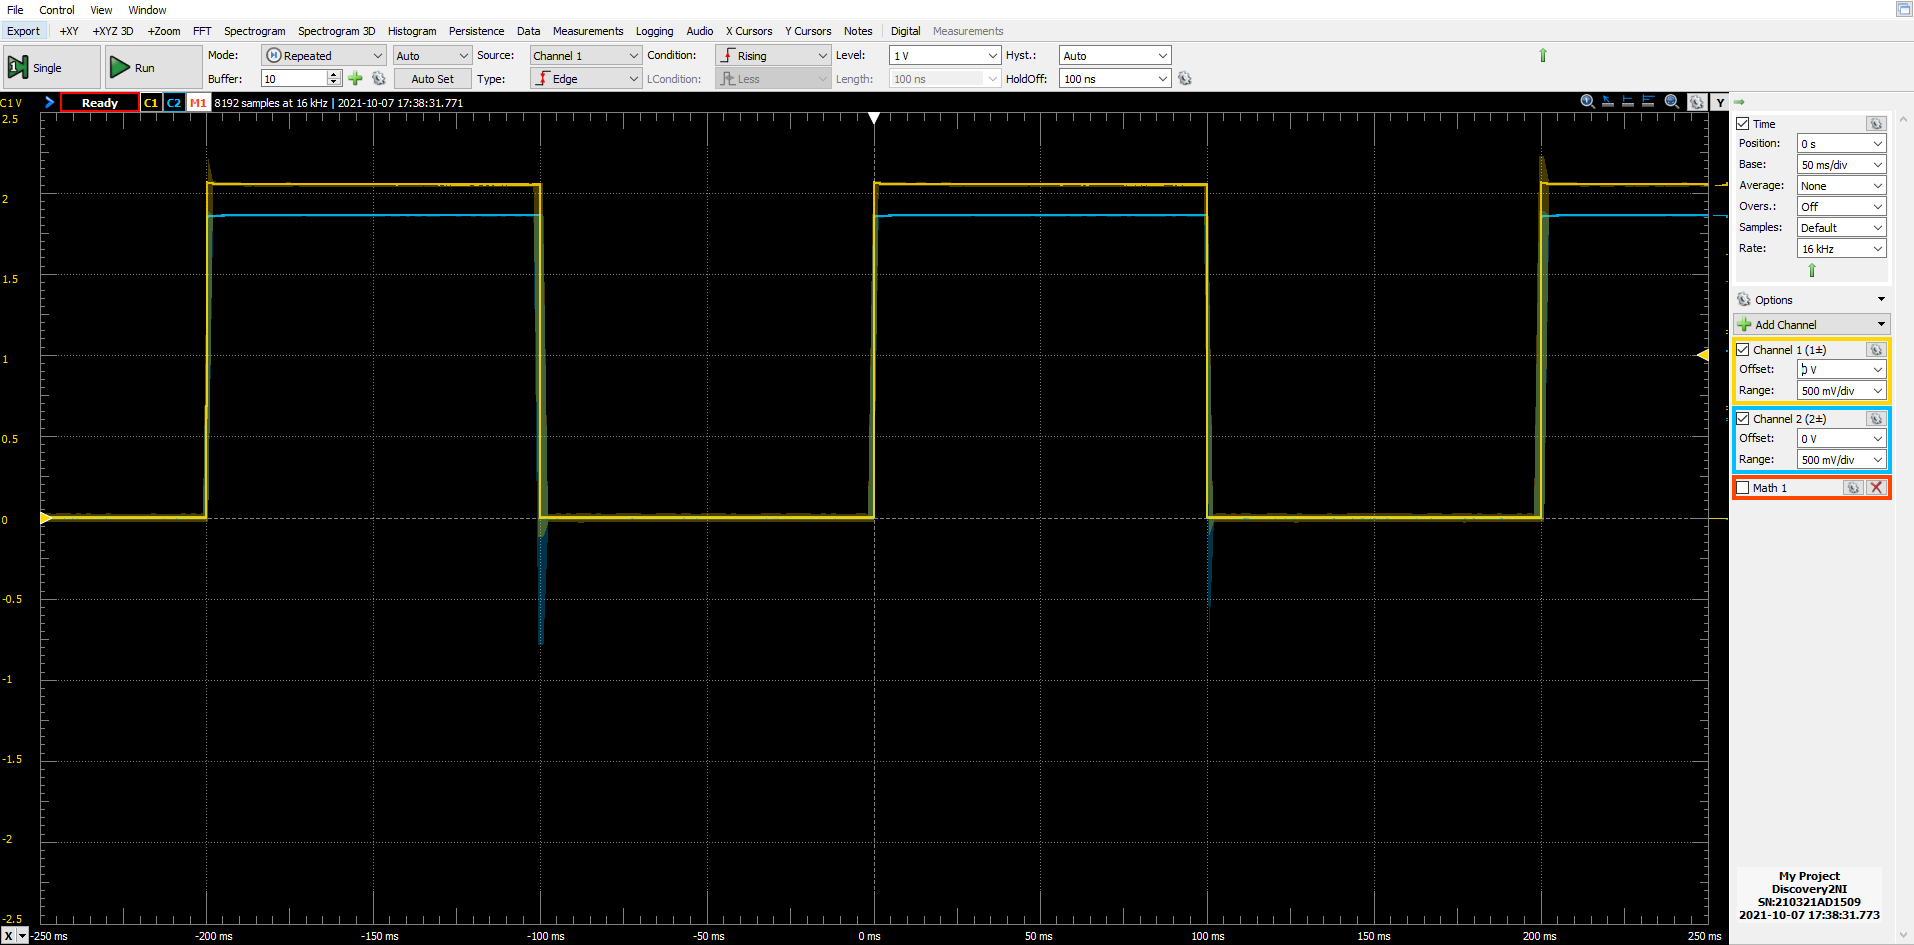
\includegraphics[scale=0.3]{sqwdiode}
\caption{(3.b) Onda quadra in ingresso $f \approx 10 \si{\Hz}$ al diodo.}
\end{figure}
\section{Oscilloscopio}

\subsection*{4.e Uso del trigger}

Quando la tensione di soglia del trigger (indicata dal triangolo giallo a
destra) incontra almeno un fronte di salita del segnale ai capi del diodo 
(CH1) la traccia rimane stabile sullo schermo. Mentre per valori di soglia
$> 2$ V o negativi la traccia viene disegnata ogni volta che il circuito di
trigger è autonomamente attivato dall'oscilloscopio, per cui il segnale sembra
spostarsi in maniera irregolare sullo schermo.

Si nota immediatamente come la tensione ai capi del diodo cresca di pari
passo con l'onda triangolare fino a quando la tensione di alimentazione 
raggiunge la tensione di soglia $V_\gamma$ del LED rosso. Una volta superata
$V_\gamma$ è la caduta di tensione sulla resistenza (CH2) a seguire il profilo
dell'onda triangolare, mentre la tensione ai capi del diodo cresce molto
lentamente; sempre secondo il modello di Shockley in maniera simile ad un
logaritmo.

\begin{figure}[htb]
\centering
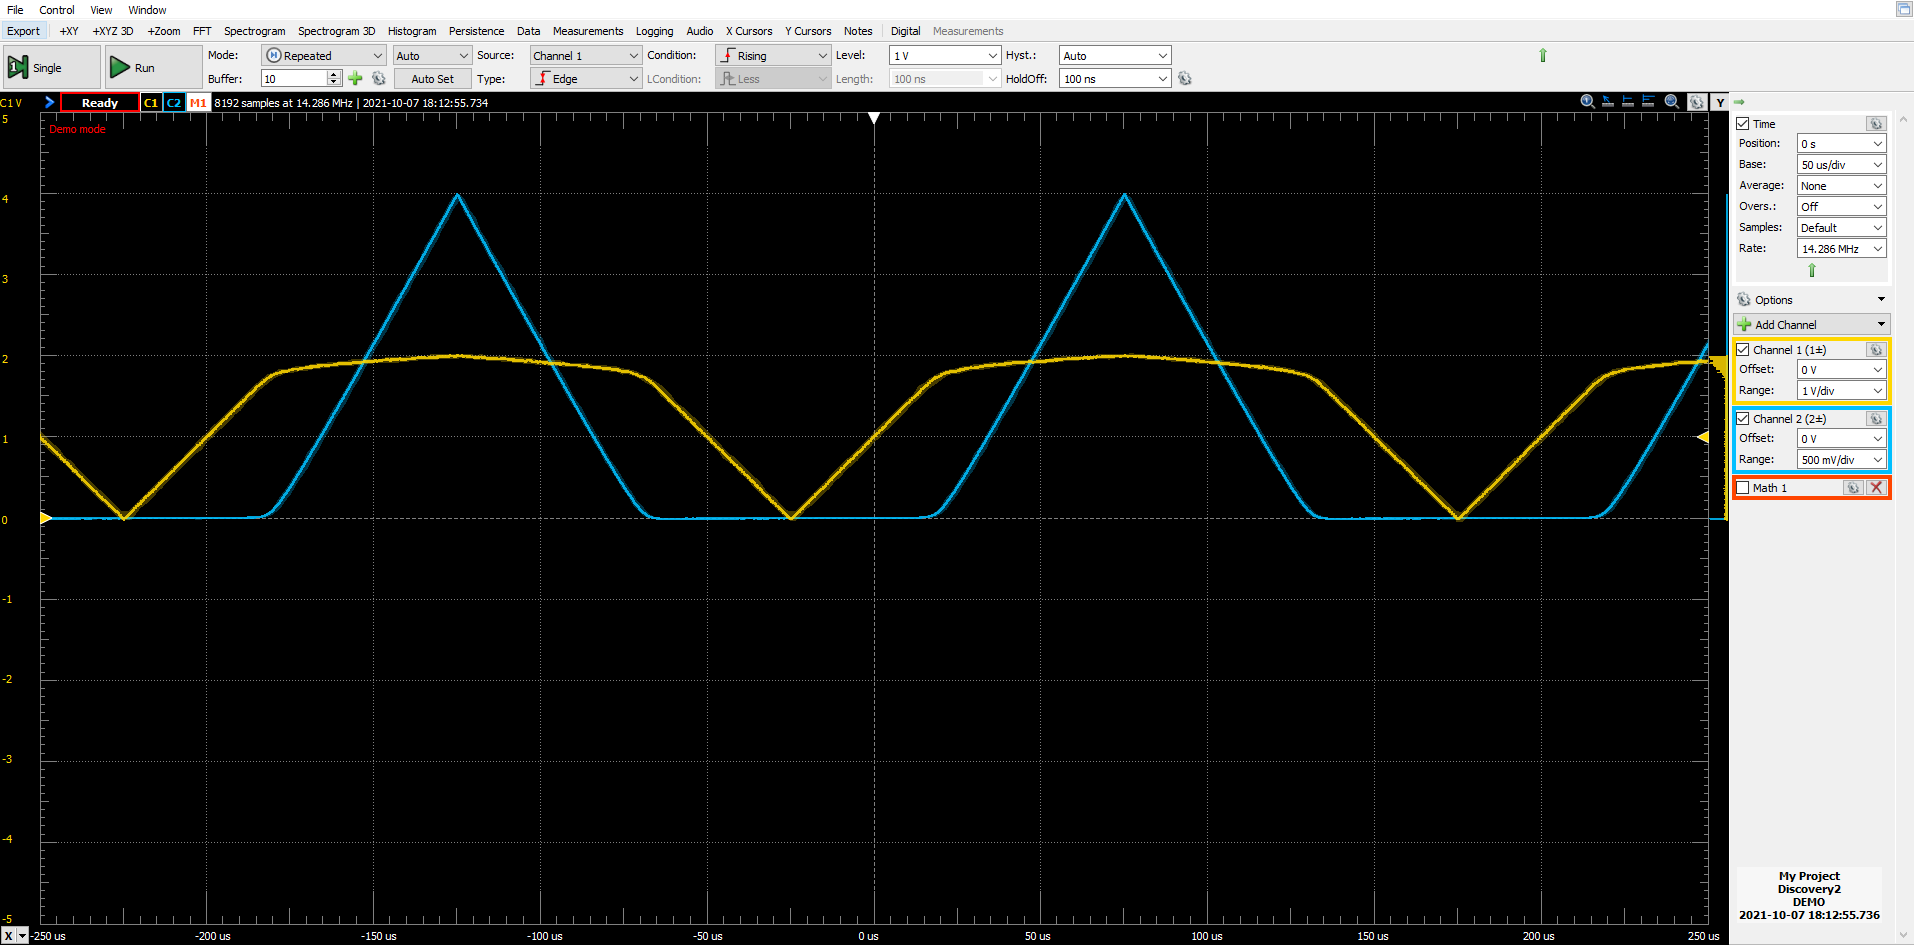
\includegraphics[scale=0.3]{trgdiode_new}
\caption{(4.e) Relazione tra trigger e segnale}
\end{figure}


\subsection*{4.f Misura tensione massima ai capi del diodo}

La tensione massima ai capi del diodo misurata con i cursori risulta essere
$V_{\mathrm{MAX}}= (2.0 \pm 0.1 ) \,\mathrm{V}$. La funzione di misura
automatica fornisce il valore $V_{\mathrm{AUTO}}= 1.975 \,\mathrm{V}$

Le due misure sono compatibili, ma la seconda è notevolmente più precisa di
quella fatta ad occhio guardando la traccia sullo schermo.


\framebox(400,30){Inserire commento sulla accuratezza della misura.}


\section{Caratteristica del diodo}
\par

\subsection*{5.c Caratteristica del diodo}

\begin{figure}[htb]
\centering
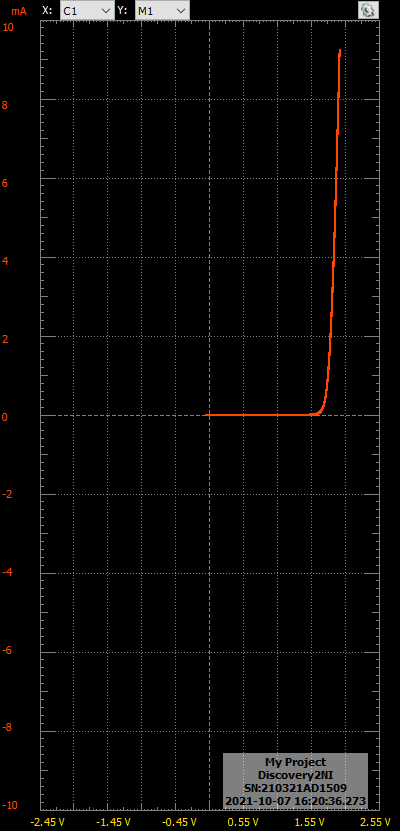
\includegraphics[scale=0.4]{shockley_new}
\caption{(5.c) Caratteristica corrente-tensione del diodo in modalit\`a XY}
\end{figure}

\subsection*{5.d Fit curva del diodo}
\par

\begin{figure}[htb]
\centering
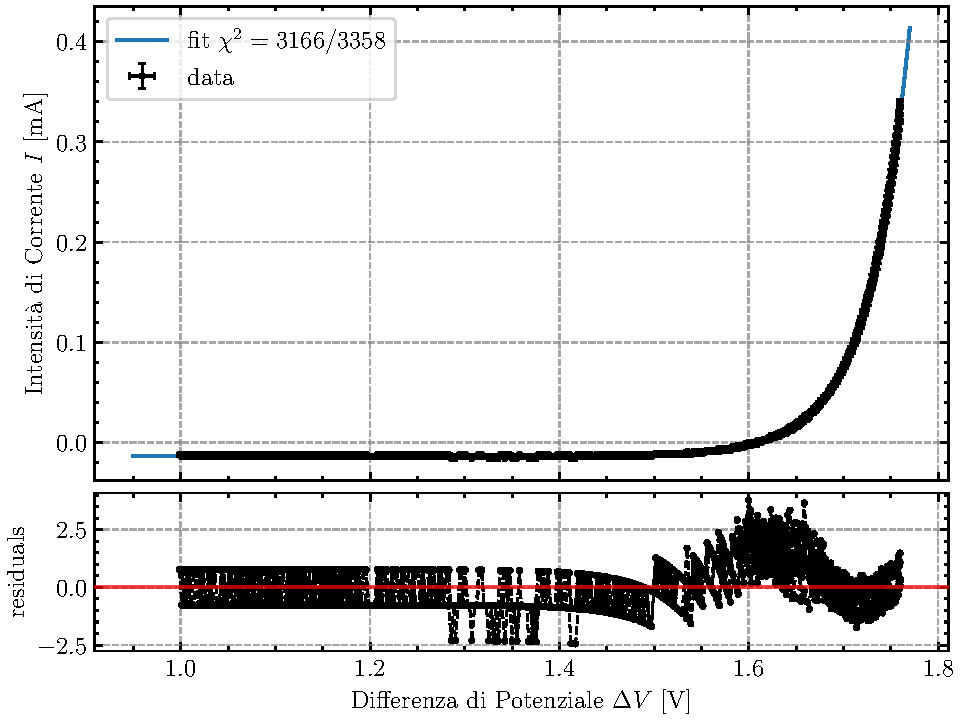
\includegraphics[scale=0.8]{ivfit}
\caption{(2.b) Grafico $I_{D}$ vs. $V_{D}$ e fit all'equazione di Schockley}
\end{figure}

\section{Partitore}

\subsection*{6.b Partitore con resistenze da 1k}

Si realizza un partitore con resistenze da $1 \,\mathrm{k}\Omega$.
Valori misurati con il multimetro: R1=$993 \pm 8 \,\Omega$,
R2=$993 \pm 8 \,\Omega$


\begin{table}[h]
\centering
\begin{tabular}{|c|c|c|c|c|c|}
\hline 
VIN& $\sigma$ VIN  & VOUT	 & $\sigma$ VOUT & VOUT/VIN & $\sigma$ VOUT/VIN \\
\hline 
1.000 & 0.005 & 0.500 & 0.003 & 0.500 & 0.008 \\
2.00 & 0.02 & 1.000 & 0.005 & 0.500 & 0.011 \\
3.00 & 0.02 & 1.500 & 0.008 & 0.500 &0.008 \\
4.00 & 0.03 & 2.00 & 0.02 & 0.500 & 0.012 \\
\hline 
\end{tabular} 
\caption{(6.b) Partitore di tensione con resistenze da circa 1k. Tutte le
tensioni in V.\label{tab:div1k}}
\end{table}

I valori di attenuazione attesi per il partitore risultano compatibili
con quelli misurati per tutti i valori di tensione compresi nell'intervallo
esplorato ($1 - 4$ V.)

\subsection*{6.d Partitore con resistenze da circa 1M}
\par
Si realizza un partitore con resistenze da $1 \,\mathrm{M}\Omega$.
Valori misurati con il multimetro: R1=$993 \pm 8 \,\mathrm{k}\Omega$,
R2=$996 \pm 8 \,\mathrm{k}\Omega$


\begin{table}[h]
\centering
\begin{tabular}{|c|c|c|c|c|c|}
\hline 
VIN& $\sigma$ VIN  &VOUT	 & $\sigma$ VOUT& VOUT/VIN & $\sigma$ VOUT/VIN \\
\hline 
1.000 & 0.005 & 0.481 & 0.003 & 0.481 & 0.008 \\
2.00 & 0.02 & 0.955 & 0.005 & 0.478 & 0.011 \\
3.00 & 0.02 & 1.431 & 0.007 & 0.477 & 0.008 \\
4.00 & 0.03 & 1.906 & 0.009 & 0.477 & 0.009 \\
\hline 
\end{tabular} 
\caption{(6.d) Partitore di tensione con resistenze da circa 1M.
Tutte le tensioni in V.\label{tab:div1M}}
\end{table}

La tensione in uscita dal partitore $R_1 + R_2$ risulta apprezzabilmente
inferiore rispetto al suo valore atteso. Questo è dovuto al comportamento
non ideale del voltmetro, per cui quando la sua impedenza in ingresso
$10 \si{\Mohm}$ (nom.) è paragonabile a quella della resistenza del partitore
a cui si trova in parallelo durante la misura, ne abbassa la resistenza
effettiva $R_2 \mapsto R_{\mathrm{eff}} = (\frac{1}{R_{\mathrm{in}}}
+ \frac{1}{R2})^{-1}$. Di conseguenza aumenta la corrente che passa per
il partitore, dunque la caduta di tensione ai capi di $R_1$, per cui
diminuiscono la tensione in uscita e quindi il valore di attenuazione, come
osservato.


\subsection*{6.e Resistenza di ingresso del multimetro}
Usando il modello mostrato nella scheda si ottiene
\begin{equation}\label{eq: divider}
\frac{R_1}{R_{IN}} =  \frac{V_{IN}}{V_{OUT}} - (1 +  \frac{R_1}{R_2} )
\end{equation}

Con i dati con resistenze da 1k si ottiene
\begin{equation}\label{eq: estimate}
R_1/R_{IN} = 0.00  \pm  0.04   \implies  R_{IN} \geq 2 \si{k\ohm}
\end{equation}


Con i dati con resistenze da 1M si ottiene
\[ R_1/R_{IN} = 0.09  \pm  0.04   \implies  R_{IN} = (11 \pm  5) \si{M\ohm}
\]

Quando la resistenza del multimetro $R_{IN} \gg R_2$ come visto al punto
6.b si ha $A \approx A_{\exp}$, per cui dalla \eqref{eq: divider}
\[
\frac{1}{A} - \frac{1}{A_{\exp}} = \frac{V_{IN}}{V_{OUT}} -
(1 +  \frac{R_1}{R_2}) = \frac{R_1}{R_{IN}}
\]
si vede come (a causa dell'incertezza sulla stima di $R_{IN}$ dalla
propagazione dell'errore sulla differenza) non sia possibile dare una misura
soddisfacente del suo valore. Ne possiamo però dare una stima dal basso:
\[
\frac{1}{A} \geq \frac{R_1}{R_{IN}} \implies R_{IN} \geq A R_1
\]
come in \eqref{eq: estimate}.

\section{Misure di tempo e frequenza}

\subsection*{7.e Misure di frequenza}
Misure con onda sinusoidale
\begin{table}[h]
\centering
\begin{tabular}{|c|c|c|c|c|c|}
\hline 
Periodo T ($\mu$ s)& $\sigma$ T ($\mu$ s) &Frequenza f (kHz) & $\sigma$ f (kHz) &
Misura oscilloscopio (kHz) & Differenza (kHz)\\
\hline 
999 & 10 & 0.99 & 0.01 & \exn &\exn \\
99.9 & 1.1 & 10.00 & 0.11 & \exn &\exn \\
9.99 & 0.10 & 100.0 & 1.0 & \exn &\exn \\
0.999 & 0.011 & 1000 & 11 & \exn &\exn \\
\hline 
\end{tabular} 
\caption{(7.e) Misura di frequenza di onde sinusoidali e confronto con
misurazione interna dell'oscilloscopio }
\end{table}

\subsection*{7.f Misure di duty cyle}
Misure con onda quadra
\begin{table}[h]
\centering
\begin{tabular}{|c|c|c|c|c|c|}
\hline 
Periodo T ($\mu$ s)& $\sigma$ T ($\mu$ s) & Durata alto $t_H$ (s) & $\sigma$ $t_H$ (s)
& Duty cycle D(\%) & $\sigma$ D (\%) \\
\hline 
100 & 2 & 9 & 2 & 0.09 & 0.02 \\
100 & 2 & 50 & 2 & 0.50 & 0.02 \\
100 & 2 & 90 & 2 & 0.90 & 0.02 \\
\hline 
\end{tabular} 
\caption{(7.f) Misura di duty cycle per onde quadre }
\end{table}


\subsection*{7.g Tempo di salita e di discesa}
Misure su onda quadra
\[
f = (1.000 \pm 0.011) \si{M\Hz}, \quad
t_\mathrm{salita} = (35 \pm 6) \mathrm{ns},
t_\mathrm{discesa} = (37 \pm 6) \mathrm{ns},
\]

La misura è un po' balorda, visto che il tempo di salita/discesa è dello
stesso ordine di grandezza del periodo di campionamento $\nicefrac{1}{f_s} = \Delta t \approx 10 \si{\ns}$.


\framebox(400,30){Inserire commento su altre caratteristiche del segnale
ed eventualmente uno screenshot}

\section{Conclusioni e commenti finali}
Si è riusciti ad apprezzare la differenza tra il comportamento ideale e quello
realmente esibito da due circuiti molto semplici. Nel primo per la non
trascurabilità dello strumento di misura sul funzionamento del partitore di
tensione (DUIT); nel secondo per la componente resistiva del diodo reale.

\section*{Dichiarazione}
I firmatari di questa relazione dichiarano che il contenuto della relazione
\`e originale, con misure effettuate dai membri del gruppo, e che tutti i
firmatari hanno contribuito alla elaborazione della relazione stessa.

\end{document}
